\documentclass {CSEThesis}
% Standard packages
\usepackage{amsmath}        % Extra math definitions
\usepackage{graphics}       % PostScript figures
\usepackage{setspace}       % 1.5 spacing
%\usepackage{psfig,epsfig}
\usepackage{multicol}
\usepackage{subfigure}
\usepackage{epsfig,color}
\usepackage{graphicx}
\usepackage{listings}
\usepackage{xcolor}
\usepackage{algcompatible}
\usepackage[]{algorithm}
\usepackage{inconsolata}
\usepackage[noend]{algpseudocode}
\usepackage[section]{placeins}
\usepackage{float}

\usepackage[english]{babel}
\usepackage{hyperref}
% for captialised first letter in references
\newcommand{\algorithmautorefname}{Algorithm}
\addto\extrasenglish{%
  \def\chapterautorefname{Chapter}%
  \def\sectionautorefname{Section}%
  \def\subsectionautorefname{Subsection}%
  \def\subsubsectionautorefname{Subsubsection}%
  \def\paragraphautorefname{Paragraph}%
  \def\subparagraphautorefname{Subparagraph}%
  \def\figureautorefname{Figure}%
  \def\algorithmautorefname{Algorithm}%
}

\usepackage{xcolor}
\hypersetup{
    colorlinks,
    linkcolor={red!50!black},
    citecolor={green!50!black},
    urlcolor={blue!80!black}
}

\graphicspath{{./images/}}

\makeatletter
\def\BState{\State\hskip-\ALG@thistlm}
\makeatother

\definecolor{darkscarlet}{rgb}{0.34, 0.01, 0.1}
\definecolor{ultramarineblue}{rgb}{0.25, 0.4, 0.96}
\definecolor{alizarin}{rgb}{0.82, 0.1, 0.26}
\definecolor{cadmiumgreen}{rgb}{0.0, 0.42, 0.24}
\definecolor{desertsand}{rgb}{0.93, 0.79, 0.69}
\lstset {
    % backgroundcolor=\color{white},   
    % commentstyle=\color{green},
    % keywordstyle=\color{blue},
    % stringstyle=\color{red},
    language=C++,
    showstringspaces=false,
    numbers=left,
    basicstyle=\footnotesize\ttfamily,
}

\newcommand{\tabf}{\;\;\;\;}
\newcommand{\tabs}{\;\;\;\;\;\;\;\;}
\newcommand{\tabt}{\;\;\;\;\;\;\;\;\;\;\;\;}
\providecommand{\tightlist}{%
  \setlength{\itemsep}{0pt}\setlength{\parskip}{0pt}}

% Custom packages
%\usepackage[first]{datestamp}   % Datestamp on first page of each chapter


\usepackage{color}
%===== page layout
% Define the side margins for a right-side page
%\insidemargin = 1.3in \outsidemargin = 0.9in
% Above margin is space above the header
% Below margin is space below footer
%\abovemargin = 1.5in \belowmargin = 0.05in


\btptitle = {Program Analysis - Herbrand Equivalence} % { and } are needed around your name
\name = {Himanshu Rai}          % and other feilds. don't remove.
\rollno = {111601032}
\email = {111601032@smail.iitpkd.ac.in}
\guide = {Dr Jasine Babu}


\begin{document}

\begin{titlepage}
\begin{center}
\textheight 15.5in \textwidth 12.5in {\large\sf  \textbf{\the\btptitle}}\\[12ex]
{\small{\textsl{ \textbf{A Project Report Submitted \\
in Partial Fulfillment of the Requirements \\
for the Degree of \\
[3ex]\small \bf Bachelor of Technology}}}}\\
[16ex] \emph{by}
\\[2ex]
{\sf \sf \textbf{\the\name}\\
             (\the\rollno)}\\[1ex]
\emph{under the guidance of}\\[2ex]
{\sf \bf \the\guide} \\[7ex]

\vspace{1.2in}

 \begin{figure}[!h]
\centering
 
\includegraphics[width=0.15\textwidth]{IITPkdFullLogoColor}
 \end{figure}



{\small\bf DEPARTMENT OF COMPUTER SCIENCE AND ENGINEERING}  \\[1ex]
%{\small \bf{INDIAN INSTITUTE OF TECHNOLOGY PALAKKAD}}
%\\[2ex]
%
%  {\color{red} \hrule height 0.5ex}
% \vskip 1ex
% May \the\year 
\end{center}
\end{titlepage}


\raggedbottom
\doublespacing
\pagenumbering{roman}
\chapter*{\centering \underline{CERTIFICATE}}
\vskip 2ex \emph{\quad This is to certify that the work contained
in this thesis entitled ``\textbf{\the\btptitle}'' 
is a bonafide work of \textbf{\the\name}
(\textbf{Roll No. \the\rollno}), carried out in the Department of
Computer Science and Engineering, Indian Institute of Technology
Palakkad under my supervision and that it has not been submitted
elsewhere for a degree.} \vskip 15ex

\begin{flushright}
	\textbf{Dr Jasine Babu}\\
	Assistant/Associate Professor \\
	Department of Computer Science \& Engineering \\
	Indian Institute of Technology Palakkad
\end{flushright}
\hfill 
\hfill 





% \chapter*{\centering Acknowledgements}
\quad Write acknowledgements, if your want to.



\tableofcontents 

\addcontentsline{toc}{chapter}{List of Figures} 
\listoffigures 

% \addcontentsline{toc}{chapter}{List of Tables} 
% \listoftables

\pagenumbering{arabic}
\def\headrulehook{\color{black}}      % Color the header rule

%========== Chapters
\typeout{}
\chapter{Introduction}
\label{chap:chapter1}
\pagenumbering{arabic}\hspace{3mm}

The basic job of a compiler is code translation from a high level 
language to a target assembly language. But, compilers also run
multiple optimization pass in the intermediate stages of translation, 
so that the finally generated code performs better than just a normal 
translated code. There might be a one time overhead of 
running optimizations, but the performance gain visible over multiple 
executions of the code outweighs it.

Modern compilers performs a large number of optimizations like
induction variable analysis, loop interchange, loop invariant code
motion, loop unrolling, global value numbering, dead code 
optimizations, constant folding and propagation, common subexpression 
elimination etc. One common feature of most of these optimizations is 
detecting equivalent program subexpressions. 

Checking equivalence of program subexpressions has been shown to be 
an undecidable problem, even when all the conditional statements are 
considered as non deterministic. So, in most of the cases compilers 
try to find some restricted form of expression equivalence. One such
form of expression equivalence is \textbf{Herbrand Equivalence} (see section \ref{sec:HerbrandEquivalence}).
Detecting equivalence of program subexpressions can be used for 
variety of applications. Compilers can use these to perform several 
of the optimizations mentioned above like constant propagation, 
common subexpression elimination etc. Program verification tools can 
use these equivalences to discover loop invariants and to verify 
program assertions. This information is also important for discovering
equivalent computations in different programs, which can be used by
plagiarism detection tools and translation validation tools \cite
{Necula, Pnueli}, which compare a program with an optimized version
in order to check correctness of the optimizer.


\section{Herbrand Equivalence}
\label{sec:HerbrandEquivalence}
A formal definition of \textbf{Herbrand Equivalence} is given in 
\cite{Ruthing}.
Informally, two expressions are \textbf{Herbrand equivalent at a program 
point}, if and only if they have syntactically the same value at that 
particular point, \textbf{across all the execution paths} from the start 
of the program which reaches that point. For the purpose of analysis, 
the operators themselves are treated as uninterprated functions with 
no semantic significance, only syntactic information is taken into 
consideration (see \ref{sec:ASimpleExample}{example below}).

For \textbf{Herbrand equivalence analysis}, we consider the set of all 
possible expressions that can be formed using the constants, 
variables and operators used in the program. And for each program 
point, partition them such that two expressions are Herbrand 
equivalent at that point if and only if they belong to the same 
partition class for that point.

\section{A Simple Example}
\label{sec:ASimpleExample}

\begin{figure}[!ht]
\label{fig:HerbrandEquivalenceTrans}
    \centering {
        \setlength{\fboxsep}{8pt}    
        \fbox{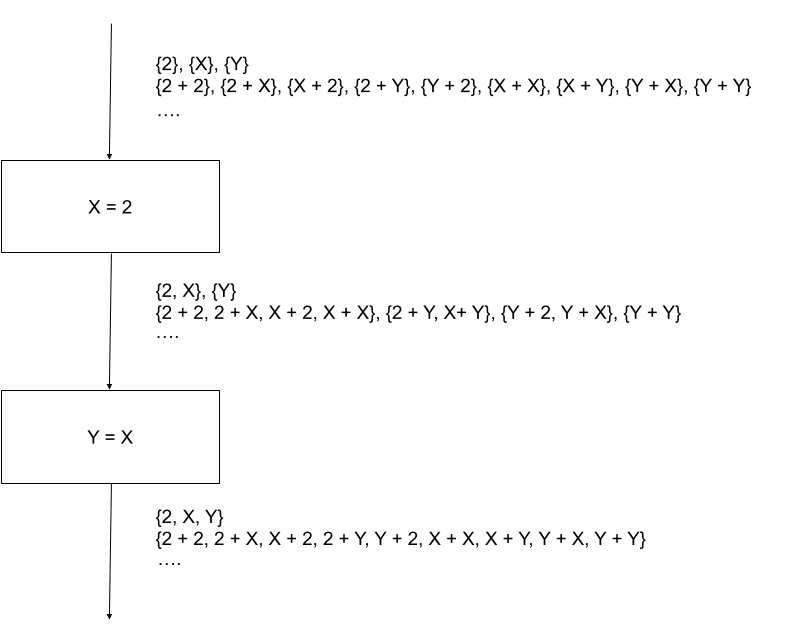
\includegraphics[scale=0.55]{HerbrandEquivalenceTrans.png}}
    }
    \caption{Example of Herbrand Equivalence}
\end{figure}

Figure \ref{fig:HerbrandEquivalenceTrans} shows a simple example of Herbrand Equivalence analysis. All the expressions that belongs to the same set at a program point are Herbrand equivalent at that point.
\begin{itemize}
    \item   Initially all the expressions are in separate sets, ie. 
    they are inequivalent to each other. In particular, note that 
    $X + 2$ and $2 + X$ are inequivalent because the operators are 
    being treated uninterprated with no semantic information of them, 
    which means there is no knowledge of commutativity of $+$.
    \item   After assignment $X = 2$, any occurrence of $X$ in an
    expression can be replaced with $2$. So, now all expressions with 
    $2$ in place of $X$ and vice versa are equivalent - that means
    $2 + 2$, $2 + X$, $X + 2$, $X + X$ are all equivalent - this still 
    is just syntactic information because $X$ and $2$ are equivalent. 
    However, if $4$ was also in the universe of expressions, $2 + 2$ and 
    $4$ are not equivalent as this is semantic information of $+$.
    \item   After assignment $Y = X$, any occurrence of $Y$ in 
    an expression can be replaced with $X$. Because $X$ and $2$ are already 
    equivalent, it means now $2$, $X$, and $Y$ are all equivalent to 
    each other. And two expressions are equivalent if one can be 
    obtained from the other by replacing one of these with any of the 
    other two. For this example, it means that two expressions of 
    the same length are equivalent.
\end{itemize}

\begin{figure}[!ht]
\label{fig:HerbrandEquivalenceConv}
    \centering {
        \setlength{\fboxsep}{8pt}    
        \fbox{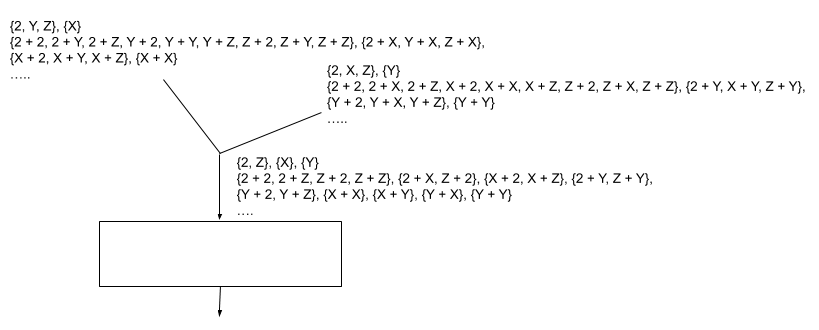
\includegraphics[scale=0.54]{HerbrandEquivalenceConv.png}}
    }
    \caption{Example of Herbrand Equivalence analysis at a confluence point}
\end{figure}

Figure \ref{fig:HerbrandEquivalenceConv} shows what happens at a 
\textbf{confluence point} - a point where multiple paths meet. Two 
expressions are Herbrand equivalent only if they are Herbrand 
equivalent at all the predecessor points.
\begin{itemize}
    \item   In the left branch $2$, $Y$, $Z$ are equivalent and 
    so are expressions which are interconvertible by replacement 
    of any of these three, with any other.
    \item   The case with the right branch is similar, except $X$ is 
    equivalent to $2$ and $Z$ instead of $Y$.
    \item   At the confluence point, only $2$ and $Z$ are equivalent 
    because they were equivalent at both the predecessors points. $X$ 
    was equivalent to $2$ and $Z$ at the right predecessor but not 
    the left one and $Y$ was equivalent to $2$ and $Z$ at the left 
    predecessor but not the right. As before, expressions obtained by 
    replacing $2$ with $Z$ and vice versa are equivalent.
\end{itemize}

\section{Goal of the Project}
\label{sec:GoalOfTheProject}
\cite{Babu} gives an algorithm for Herbrand Equivalence analysis
restricted to program expressions. The basic goal of this project 
is to refine this general algorithm and then implement it for 
\href{https://llvm.org/}{Clang-LLVM compiler}; then extend this 
algorithm to use the analysis information for performing actual program
optimizations. Finally, a proof of correctness of the algorithm has 
to be presented which would also be based on the work in \cite{Babu}.

\section{Organization of the Report}
\label{sec:OrganizationOfTheReport}
Chapter \ref{chap:chapter2} gives a brief overview of previous works 
related to the Herbrand Equivalence; then summary of the 
papers \cite{Gulwani, Saleena, Babu} are specifically presented. Chapter 
\ref{chap:chapter6} provides a tutorial on writing an LLVM 
optimzation pass. Chapter \ref{chap:chapter7} gives pseudocode for Herbrand 
Equivalence analysis of a program; algorithms in chapter \ref{chap:chapter8} 
extends these to use the analysis information for performing actual program 
optimizations.

\cleardoublepage 
\typeout{}
\chapter{Review of Prior Works}
\label{chap:chapter2}

Existing algorithms for calculating Herbrand Equivalence are either
exponential or are imprecise. The precise algorithms are based on an 
early algorithm by Kildall \cite{Kildall}, which discovers 
equivalences by performing an abstract interpretation over the 
lattice of Herbrand equivalences. Kildall algorithms is precise in 
the sense it finds all the Herbrand equivalences but is exponential 
in time. The partition refinement algorithm of Alpern, Wegman and 
Zadek (AWZ) \cite{AWZ} is efficient but is much imprecise compared to 
Kildall's. AWZ algorithm represent the values of variables after a 
join using a fresh selection function $\phi_i$, similar to functions 
in the static single assignment form and treats $\phi_i$ as 
uninterpreted functions. It is incomplete in the sense it treats all 
$\phi_i$ as uninterpreted. In an attempt to remedy this problem, 
Ruthing, Knoop and Steffen proposed a polynomial-time algorithm (RKS) 
\cite{RKS} that alternately applies the AWZ algorithm and some 
rewrite rules for normalization of terms involving $\phi$ functions, 
until the congruence classes reach a fixed point. Their algorithm 
discovers more equivalences than the AWZ algorithm, but remains 
incomplete. 

Gulwani and Necula \cite{Gulwani} gave algorithm to find the Herbrand 
Equivalence classes restricted to program expressions. There 
algorithm is linear in parameter $s$, where $s$ is the maximum times 
operators occur in a program expression. Clearly $s$ can take a maximum 
value of $n$, which is the program size, so the algorithm in all is 
polynomial in $n$. Later, Saleena and Paleri \cite{Saleena} showed  
that Gulwani's algorithm losses some information as it removes a 
equivalence class if it does not contain a variable or a constant. 
The global value numbering (GVN) algorithm proposed by them was able 
to detect more redundencies compared to that by Gulwani and Necula.

One problem is that most of these alogrithms were based on fix point 
computations but the classical definition of Herbrand equivalence is 
not a fix point based definition making it difficult to prove their 
precision or completeness. Babu, Krishnan and Paleri \cite{Babu} 
developed a lattice theoretic fix-point formulation of Herbrand 
Equivalence on the lattice defined over the set of all terms 
constructible from variables, constants and operators of a program. 
They showed this definition is equivalent to the classical meet over 
all path characterization over the set of all possible expressions. 
The algorithm proposed by them is able to detect all the equivalences 
as by that of Saleena and Paleri.

So, to sum up Kildall's algorithm finds all the equivalent classes 
but is exponential. The algorithms by Saleena and Paleri; Babu, 
Krishnan and Paleri are polynomial and efficient among other 
imprecise algorithms. They are able to find all equivalence classes 
restricted to program expressions (all expressions with length atmost 
2), which is precisely what is practically useful.
\cleardoublepage 
\typeout{}
\chapter{Summary of Gulwani and Necula}
\label{chap:chapter3}

Gulwani showed that there is a family of acyclic programs for which 
the set of all Herbrand equivalences requires requires an exponential 
sized (with respect to the size of the program) value graph 
representation - the data structure used by Kildall in his algorithm. 
He also showed that Herbrand Equivalences among program sub 
expressions can always be represented using linear sized value graph. 
This explains the reason for exponential complexity of Kildall's 
algorithm which cannot be improved to polynomial and imprecise nature 
of existing polynomial time algorithms.

So contrasting to Kildall's algorithm, which finds \textit{all the 
Herbrand Equivalent classes} corresponding to constants, variables 
and operators occurring in the program, Gulwani's algorithm discovers 
\textit{equivalences among program subexpressions} (expressions that 
can occur syntactically in a program), in linear time with respect to 
parameter $s$, the maximum size of an expression in terms of number 
of operators used. For global value numbering, $s$ can be safely 
taken to be $N$, the size of the program and hence the algorithm is 
linear in the program size.

Also, he proved that the lattice of sets of Herbrand equivalences has 
finite height $k$, which is the number of program variables. So, an 
abstract interpretation over the lattice of Herbrand equivalences 
will terminate in at most $k$ iterations even for cyclic programs.

\section{Brief overview of the algorithm}
The program expressions considered can be represented as
$$e\; ::=\; x\: |\: c\: |\:F(e_1, e_2)$$
Here, $c$ and $x$ are constants and variables occurring in the 
program.

The data structure used is called \textit{Strong Equivalence DAG 
(SED)}. Each node is of the form $<V,t>$ where $V$ is a set of 
program variables and $t$ is either $\perp$ or $c$ for leaf nodes and 
$F(n_1, n_2)$ where $n_1$ and $n_2$ are SED nodes for non leaf nodes
(also indicating that the node has two ordered successors). $\perp$ 
means that the variables in the node have undefined values.

There is a SED associated with each program point and the algorithm
starts with the following initial SED
$$G_0\; =\; \{<x,\perp>\: |\: x \text{ is a program variable}\}$$ 
Two functions $Join(G_1, G_2, s')$ and $Assignment(G_1, x := e)$ are 
used to compute SEDs for other points in the flow graph node 
corresponding to the program, as shown in figure 
\ref{fig:GulwaniAlgorithm}. $s'$ in the argument of \textit{Join} is 
a positive integer, and it returns equivalences between expressions of
size atmost $s'$.

\begin{figure}[!h]
    \centering {
        \setlength{\fboxsep}{8pt}    
        \fbox{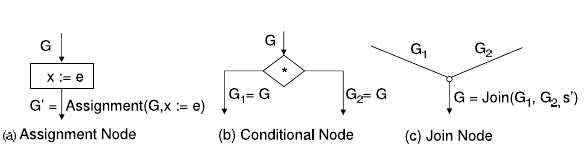
\includegraphics[scale=0.5]{GulwaniAlgorithm.png}}
    }
    \caption{Computation of SED for flowgraph nodes of a program}
    \label{fig:GulwaniAlgorithm}
\end{figure}

For detailed implementation of \textit{Join} and \textit{Assignment} 
and correctness proof of the algorithm, see \cite{Gulwani}.

\section{Complexity of the algorithm}
The complexity of the algorithm is $O(k^{3} * N * j)$, where $k$ is  
the total number of program variables, $N$ is the size of the program 
and $j$ is the number of join operations in the program. $k$ and $j$ 
are bounded by $N$, making the whole algorithm polynomial in $N$.
\cleardoublepage 
\typeout{}
\chapter{Algorithm for Herbrand Analysis}
\label{chap:chapter4}

This chapter presents an algorithm for Herbrand analysis. The pseudocode  
mentioned here is an updated version of the algorithm mentioned in \cite{Babu} 
for Herbrand equivalence analysis. The corresponding implementation done for 
LLVM compiler framework and a toy language can be found on 
\href{https://www.github.com/himanshu520/HerbrandEquivalence}{GitHub}.
Also, see \autoref{chap:chapter7} and \autoref{chap:chapter8} for more details.

One important distinction must be clear between the general Herbrand analysis problem
and the one that the algorithm in this chapter addresses. The universe for the Herbrand 
equivalence problem is the set of all expressions that can be formed using constants, 
variables and operators used in the program. But as already mentioned, the algorithm 
here is concerned with a restricted universe - set of expressions of length atmost two 
formed using constants, variables and operators in the program. 

\section{Notation}
\label{sec:NotationPseudocode}

Let $\mathcal C$ and $\mathcal X$ be the set of constants and variables used in the program;
$\mathcal W$ be our working set, which is the set of all expressions of length at most two 
that can be formed using ($\mathcal C \cup \mathcal X$). Also, $V$ be the set of all program 
points, with a special point \texttt{START} denoting the beginning of the program.
\bigbreak \noindent Three global variables are maintained - 
\begin{itemize} \tightlist
    \item \texttt{Partitions} : It is two-dimensional integer array indexed by the 
                                elements of sets $V$ and $\mathcal W$ respectively. It 
                                helps to keep track of partitions at some $v \in V$ by
                                holding same integer at \texttt{Partitions[$v$][$e$]} and
                                \texttt{Partitions[$v$][$e'$]}, for $e, e' \in \mathcal W$ 
                                if they belongs to the same equivalence class at $v$.
                                Basically, the array maintains set identifiers which helps 
                                to identify whether two expressions belong to the same sets 
                                (equivalence classes).
    \item \texttt{SetCnt} : It helps to keep track of the next set identifier (an integer)
                            to be used. Whenever, a set identifier is needed the current 
                            value of \texttt{SetCnt} is used and at the same time it is 
                            incremented so that the same number is never used again.
    \item \texttt{Parent} : It is \texttt{map} indexed by a tuple of three elements - an   
                            operator and two set identifiers. Whenever an expression 
                            ($x + y$) is assigned a set identifier $c$, $c$ is stored in 
                            \texttt{Parent} with $\{+, a, b\}$ as key, where $a$ and $b$ are 
                            the set identifiers of $x$ and $y$ respectively. Next time 
                            when a set identifier for an expression ($x' + y'$) is needed, 
                            where $x'$ and $y'$ have identifiers $a$ and $b$ respectively, 
                            $c$ is used instead of using a new set identifier - the \texttt
                            {Parent} of $\{+, a, b\}$ that was earlier stored in the map.
\end{itemize}

\bigbreak \noindent There are a few functions whose definitions are not required explicitly - 
\begin{itemize} \tightlist
    \item \texttt{OPERATOR($e$)} : Returns operator used in expression $e \in (\mathcal W \setminus (\mathcal C \cup \mathcal X))$
    \item \texttt{LEFT($e$)} : Returns left operand of expression $e \in (\mathcal W \setminus (\mathcal C \cup \mathcal X))$
    \item \texttt{RIGHT($e$)} : Returns right operand of expression $e \in (\mathcal W \setminus (\mathcal C \cup \mathcal X))$
    \item \texttt{PREDECESSORS($v$)} : Returns the set of predecessors of program point $v \in V$
\end{itemize}

\bigbreak \noindent \textbf{NOTE} - For implementation, the identifiers corresponding to 
$\top$ partition should be such that they don't occur in normal partitions and are also 
easily distinguishable from them. An easy choice for consistency is to use non-negative 
integers as normal set identifiers and an array of -1 to refer $\top$ partition.

\section{Pseudocode}
\label{sec:Pseudocode}

\begin{algorithm}
    \caption{Main Herbrand Equivalence Analysis Function}
    \label{alg:HerbrandEquivalenceAnalysis}
    \begin{algorithmic}
        \Procedure{HerbrandAnalysis}{$ $}
            \State \Comment{\% Initialise \texttt{Partitions} for all program points \%}
            \For{$v \in V$}
                \State \texttt{Partitions[$v$]} $\gets \top$
            \EndFor
            \State \Comment{\% Update \texttt{Partitions} for \texttt{START} point \%}
            \State \Call{findInitialPartition}{$ $}
            \State \Comment{\% Process all program points till convergence \%}
            \State \textbf{converged} $\gets$ \texttt{false}
            \While{\texttt{converged} \textit{is False}}
                \State \texttt{converged $\gets$ true}
                \For{$v \in (V \setminus \{\texttt{START}\})$}
                    \State \textbf{oldPartition} $\gets$ \texttt{Partitions[$v$]}
                    \State \Comment{\% Update \texttt{Partitions} at $v$ \%}
                    \If{$v$ \textit{is a Transfer Point}}
                        \State \Call{TransferFunction}{$v$}
                    \Else
                        \State \Call{ConfluenceFunction}{$v$}
                    \EndIf
                    \State \Comment{\$ Update \texttt{convergence} flag \%}
                    \If{\textit{not} \Call{SamePartition}{\texttt{oldPartition, Partitions[$v$]}}}
                        \State \texttt{converged $\gets$ false}
                    \EndIf
                \EndFor
            \EndWhile
        \EndProcedure
    \end{algorithmic}
\end{algorithm}

\begin{algorithm}
    \caption{Transfer Function}
    \label{alg:TransferFunction}
    \begin{algorithmic}
        \Procedure{TransferFunction}{$v : x \gets e$}
            \State \textbf{u} $\gets$ \Call{Predecessors}{$v$}
            \State \texttt{Partitions[$v$] $\gets$ Partitions[$u$]}
            \State \Comment{\% Update set identifier for $x$ \%}
            \If{$e$ \textit{is Deterministic}}
                \State \texttt{Partitions[$v$][$x$] $\gets$ Partitions[$v$][$e$]}
            \Else 
                \State \texttt{Partitions[$v$][$x$] $\gets$ SetCtr++}
            \EndIf
            \State \Comment{\% Update set identifiers for expressions containing $x$ \%}
            \For{$\{e' \in (\mathcal W \setminus (\mathcal C \cup \mathcal X)) \mid x \in e'\}$}
                \State \texttt{Partitions[v][$e'$]} $\gets$ \Call{GetSetId}{$v$, $e'$}
            \EndFor
        \EndProcedure
    \end{algorithmic}
\end{algorithm}

\begin{algorithm}
    \caption{Confluence Function}
    \label{alg:ConfluenceFunction}
    \begin{algorithmic}
        \Procedure{ConfluenceFunction}{$v$}
            \State \Comment{If all predecessor partitions are $\top$ then current partition will also be $\top$}
            \State \textbf{continueFlag} $\gets$ false
            \For{$u \in$ \Call{Predecessors}{$v$}}
                \If{\texttt{Partitions[$u$] $\neq \top$}}
                    \State \texttt{continueFlag $\gets$ true}
                \EndIf
            \EndFor
            \State
            \If{\texttt{continueFlag} \textit{is False}}
                \State \texttt{Partitions[$v$] $\gets \top$}
                \State \Return{}
            \EndIf
            \State \Comment{\texttt{accessFlag} keeps track of processed expressions}
            \For{$e \in \mathcal W$}
                \State \textbf{accessFlag}[$e$] $\gets$ \texttt{false}
            \EndFor
            \State \Comment{Process all expressions if they are still unprocessed}
            \For{$e \in \mathcal W$}
                \If{\texttt{accessFlag[$e$]} \textit{is False}}
                    \State \Comment{\texttt{PredIDs} is the set of set identifiers of $e$ at its predecessors}
                    \State \textbf{PredIDs} $\gets \phi$
                    \For{$u \in$ \Call{Predecessors}{$v$}}
                        \If{\texttt{Partitions[u] $\neq \top$}}
                            \State \texttt{PredIDs $\gets$ (PredIDs $\cup$ Partitions[$u$][$e$])}
                        \EndIf
                    \EndFor
                    \State
                    \If{\texttt{PredIDs} \textit{is Singleton}}
                        \State \texttt{Partitions[$v$][$e$] $\gets$ PredIDs}
                        \State \texttt{accessFlag[$e$] $\gets$ true}
                    \Else
                        \State \Comment{\texttt{expClass} holds $e' \in \mathcal W$ that are equivalent to $e$ at all predecessors of $v$}
                        \State \textbf{expClass} $\gets \mathcal W$
                        \For{$u \in$ \Call{Predecessors}{$v$}}
                            \If{\texttt{Partitions[u] $\neq \top$}}
                                \State \texttt{expClass $\gets$ (expClass} $\cap$ \Call{GetClass}{$u$, $e$})
                            \EndIf
                        \EndFor
                        \State \Comment{Update \texttt{Partitions} map}
                        \State \textbf{newSetID} $\gets$ \texttt{SetCnt++}
                        \For{\texttt{$e' \in$ expClass}}
                            \State \texttt{Partitions[$v$][$e'$] $\gets$ newSetID}
                            \State \texttt{acessFlag[$e'$] $\gets$ true}
                        \EndFor
                    \EndIf
                \EndIf
            \EndFor
            \State
            \State \Comment{Update \texttt{Parent} map}
            \For{$e \in (\mathcal W \setminus (\mathcal C \cup \mathcal X))$}
                \State \textbf{op} $\gets$ \Call{Operator}{$e$}
                \State \textbf{leftSetID} $\gets$ \texttt{Partitions}[\Call{Left}{$e$}]
                \State \textbf{rightSetID} $\gets$ \texttt{Partitions}[\Call{Right}{$e$}]
                \State \texttt{Parent[\{op, leftSetID, rightSetID\}] $\gets$ Partitions[v][$e$]}
            \EndFor
        \EndProcedure
    \end{algorithmic}
\end{algorithm}

\begin{algorithm}
    \caption{Checks whether two partitions are same or not}
    \label{alg:SamePartition}
    \begin{algorithmic}
        \Procedure{SamePartition}{\texttt{first, second}}
            \For{$e \in \mathcal W$}
                \If{\Call{GetClass}{\texttt{first}, $e$} $\neq$ \Call{GetClass}{\texttt{second}, $e$}}
                    \State \Return{\texttt{false}}
                \EndIf
            \EndFor
            \State \Return{\texttt{true}}
        \EndProcedure
    \end{algorithmic}
\end{algorithm}

\begin{algorithm}
    \caption{Finds equivalence class of an expression in a partition}
    \label{alg:GetClass}
    \begin{algorithmic}
        \Procedure{GetClass}{\texttt{partition}, $e$}
            \State \textbf{expClass} $\gets \phi$
            \For{$e' \in \mathcal W$}
                \If{\texttt{partition[$e'$] == partition[$e$]}}
                    \State \texttt{expClass $\gets$ (expClass $\cup$ $\{e'\}$)}
                \EndIf
            \EndFor
            \State \Return{\texttt{expClass}}
        \EndProcedure
    \end{algorithmic}
\end{algorithm}

\begin{algorithm}
    \caption{Initialises partition for START point}
    \label{alg:FindInitialPartition}
    \begin{algorithmic}
        \Procedure{FindInitialPartition}{$ $}
            \For{$x \in (\mathcal C \cup \mathcal X)$}
                \State \texttt{Partitions[START][$x$] $\gets$ SetCtr++}
            \EndFor
            \For{$e \in (\mathcal W \setminus (\mathcal C \cup \mathcal X))$}
                \State \texttt{Partitions[START][$e$]} $\gets$ \Call{GetSetID}{\texttt{Partitions[START], $e$}}
            \EndFor
        \EndProcedure
    \end{algorithmic}
\end{algorithm}

\begin{algorithm}
    \caption{Finds and returns set identifier for a two length expression in a partition, by
             looking at its operands and operator}
    \label{alg:GetSetID}
    \begin{algorithmic}
        \Procedure{GetSetID}{\texttt{partition, $e$}}
            \State \textbf{op} $\gets$ \Call{Operator}{$e$}
            \State \textbf{leftSetID} $\gets$ \texttt{partition}[\Call{Left}{$e$}]
            \State \textbf{rightSetID} $\gets$ \texttt{partition}[\Call{Right}{$e$}]
            \State
            \If{\textit{not defined} \texttt{Parent[\{op, leftSetID, rightSetID\}]}}
                \State \texttt{Parent[\{op, leftSetID, rightSetID\}] $\gets$ SetCtr++}
            \EndIf 
            \State
            \State \Return{\texttt{Parent[\{op, leftSetID, rightSetID\}]}}
        \EndProcedure
    \end{algorithmic}
\end{algorithm}

\section{Updates Over Original Algorithm}
\label{sec:UpdatesOverOriginalAlgorithm}
Following major improvements/corrections have been made to the original algorithm 
mentioned in \cite{Babu}.
\begin{itemize} \tightlist
    \item \textbf{Representing Partitions}\\
    The original algorithm uses \texttt{ID structure} to maintain equivalence information. A two-dimensional array \texttt{Partitions} having an entry for each program point and each expression, stores a pointer to an \texttt{ID object}. At a program point, two expressions are equivalent if they contain pointers to the same object. Though this approach is correct, it adds a lot of overhead in the implementation both in terms of time and space - the \texttt{ID object}s have to be created and destroyed during runtime, their data fields have to be maintained properly etc.\\
    The updated algorithm solves this problem by using just integer set identifiers instead of pointers to some dynamically created objects and the \texttt{Parent map}. Again same as before, two expressions are equivalent at a program point if \texttt{Partitions} array stores same set identifiers for the expressions at that program point. \texttt{Parent} map captures the relation between the set identifiers. This modification makes the actual implementation to be more simpler, efficient and intuitive.
    \item \textbf{Confluence Function}\\
    The \texttt{Confluence} function in the original algorithm processes only the set $\mathcal C \cup \mathcal V$ in its main loop. This is wrong and instead the whole working set $\mathcal W$ should be considered.\\
    As an example, consider the test case in \autoref{sec:tc15}. At the confluence point, $y$ and $x + 2$ must be equivalent, but the original algorithm assigns them pointers to different \texttt{ID objects} indicating they are not equivalent.
    \item \textbf{Non-deterministic Assignment}\\
    Non-deterministic assignment need not be handled separately and a single transfer function is sufficent (see \autoref{alg:TransferFunction}).
\end{itemize}

\cleardoublepage 
\typeout{}
\chapter{Summary of Babu, Krishnan and Paleri}
\label{chap:chapter5}

One of the problems with other former approaches to Herbrand 
equivalence is that most of the alogrithms were based on fix point 
computations. But the classical definition of Herbrand equivalence is 
not a fix point based definition making it difficult to prove their 
precision or completeness. Babu, Krishnan and Paleri \cite{Babu} gave 
a new lattice theoretic formulation of Herbrand equivalences and 
proved its equivalence to the classical version.

The paper defines a congruence relation on the set of all possible 
expressions and shows that the set of all congruences for a complete 
lattice. Then for a given dataflow framework with $n$ program points, 
a continuous composite transfer function is defined over the n-fold 
product of the above lattice such that the maximum fix point of the 
function yields the set of Herbrand equivalence classes at various 
program points. Finally, equivalence of this approach to the 
classical meet over all path definition of Herbrand Equivalence is 
established.

Below is a brief summary of the developments in the paper, for more 
detailed approach and proofs and for equivalence to MOP  
characterization refer to \cite{Babu}.

\section{Program Expressions}

Let $C$ and $X$ be the set of constants and variables occurring in 
the program respectively. The program expressions (terms) can be 
described as 
$$t\; ::=\; c\; |\; x\; |\; t_1 + t_2$$
where $c \in C$ and $x \in X$.

\section{Congruence Relation}
Let $T$ be the set of all program terms. A partition $P$ of terms in $T$ is said to be a congruence (of terms) if 
\begin{itemize}
    \item For $t$, $t'$, $s$, $s'$ $\in$ $T$, $t' \cong t$ and $s' \cong s$ iff $t' + s' \cong t + s$. 
    \item For $c \in C$, $t \in T$, if $t \cong c$ then either $t = c$ or $t \in X$.
\end{itemize}
Let $G(T)$ be the set of all congruences over $T$. We say $P_1 
\preceq P_2$ for $P_1, P_2 \in G(T)$, if 
$\forall A_1 \in P_1, \exists A_2 \in P_2$ such that 
$A_1 \subseteq A_2$. We define \textit{confluence} operation as 
$$P_1 \land P_2\; =\; \{A_i \cap B_j\: |\: A_i \in P_1 \text{ and } B_j \in P_2\}$$
Now, we extend $G(T)$ to $\overline{G(T)}$ by introducing abstract 
congruence $\top$ satisfying 
$P \land \top = \top, \forall P \in \overline{G(T)}$.
Also, we denote the congruence in which every element is in a 
separate class as $\bot$. 

$(\overline{G(T)}, \preceq, \bot, \top)$ 
forms a complete lattice, with $\land$ as meet operator.

\section{Transfer function}
An assignment $y := \beta$ transforms a congruence $P$ to another 
congruence $P'$. This can be described in the form of transfer 
function $f_{y = \beta}:G(T) \to G(T)$, given by
\begin{itemize}
    \item $B_i = \{t \in T\ |\ t[y \leftarrow \beta] \in A_i\}, \text{ for each } A_i \in P$
    \item $f_{y = \beta}(P) = \{B_i\ | \ B_i \neq \phi\}$
\end{itemize}
We extend this definition to form extended transfer function, 
$\overline{f}_{y=\beta} : \overline{G(T)} \to \overline{G(T)}$ 
by defining $\overline{f}_{y=\beta}(\top)\ =\ \top$, otherwise $\overline{f}_{y=\beta}(P) = f_{y=\beta}(P)$.
The extended transfer function is distributive, monotonic and continuous.

\section{Non deterministic assignment}
An assignment $y := *$ transforms a congruence $P$ to another 
congruence $P'$. This can be described in the form of another 
transfer function $f_{y = *}:G(T) \to G(T)$, given by: 
for every $t$, $t' \in T$, $t \cong_{f(P)} t'$, (here $f(P) = f_{y = *}(P)$ for simplicity) iff
\begin{itemize}
    \item $t \cong_P t'$
    \item $\forall \beta \in (T \setminus T(y)),\ t[y \leftarrow \beta] \cong_p t'[y \leftarrow \beta]$
\end{itemize}
As before we extend this transfer function to 
$\overline{f}_{y=*} : \overline{G(T)} \to \overline{G(T)}$ by defining
$\overline{f}_{y=*}(\top)\ =\ \top$, otherwise 
$\overline{f}_{y=*}(P) = f_{y=*}(P)$. 
The function $\overline{f}_{y=*}$ is also continuous.

\section{Dataflow analysis Framework}
A dataflow framework over $T$ is $D = (G, F)$ where $G(V, E)$ is the 
control flow graph associated with the program and $F$ is a 
collection of transfer function associated with program points.

\section{Herbrand Equivalence}
The Herbrand Congruence function $H_D : V(G) \to \overline{G(T)}$ 
gives the Herbrand Congruence associated with each program point and 
is defined to be the maximum fix point of the \textit{continuous
composite transfer function} 
$f_D : \overline{G(T)}^n \to \overline{G(T)}^n$, where 
$\overline{G(T)}^n$ is the product lattice, $f_D$ is a function satisfying $\pi_k \circ f_D = f_k$. Here $\pi_k$ is the projection map
and $f_k : \overline{G(T)}^n \to \overline{G(T)}$ is defined as follows 
\begin{itemize}
    \item   If k = 1, the entry point of the program $f_k = \bot$.
    \item   If k is a function point with $Pred(k) = \{j\}, \text{ then } f_k = h_k \circ \pi_j$ where 
    $h_k$ is the extended transfer function corresponding to function point k.
    \item   If k is a confluence point with $Pred(k) = {i, j}, \text{ then } f_k = \pi_{i, j}, \text{ where }
    \pi_{i, j}:\overline{G(T)}^n \to \overline{G(T)}$ is given by $\pi_{i,j}(P_1,\ \dots,\ P_n) = P_i \land P_j$.
\end{itemize}.
\cleardoublepage
\typeout{}
\chapter{Implementation Platform - Clang/LLVM}
\label{chap:chapter6}

A modern compiler has three basic components - frontend, optimiser and backend.
The frontend takes the high level source code and outputs the intermediate 
representation (IR) which serves as the input for the optimiser. The optimiser 
modifies the IR to make it more simpler and efficient - this new modified IR is 
then fed into the backend which gives the final low level code.

LLVM is a complete compiler infrastructure - a collection of libraries built to 
support compiler development and related tasks. Each library supports a particular 
component in a typical compiler pipeline - lexing, parsing, optimizations of a 
particular type, machine code generation for a particular architecture, etc. The 
central part of the LLVM project are \textbf{LLVM intermediate representation 
(LLVM IR)} and \textbf{LLVM core}. LLVM IR is the intermediate representation 
used in the LLVM project and LLVM core is responsible for all the optimisations
and transformations that happens on the IR. The most important thing about the 
project is it provides all the facilities for anyone to write their own 
optimisations.

Clang is a compiler frontend for the C family of programming languages 
(\texttt{C, C++, Objective-C} etc.). It builds on the LLVM optimizer and code 
generator, allowing it to provide high-quality optimization and code generation 
support for many targets.

\begin{figure}[!t]
  \centering {
      \setlength{\fboxsep}{8pt}    
      \fbox{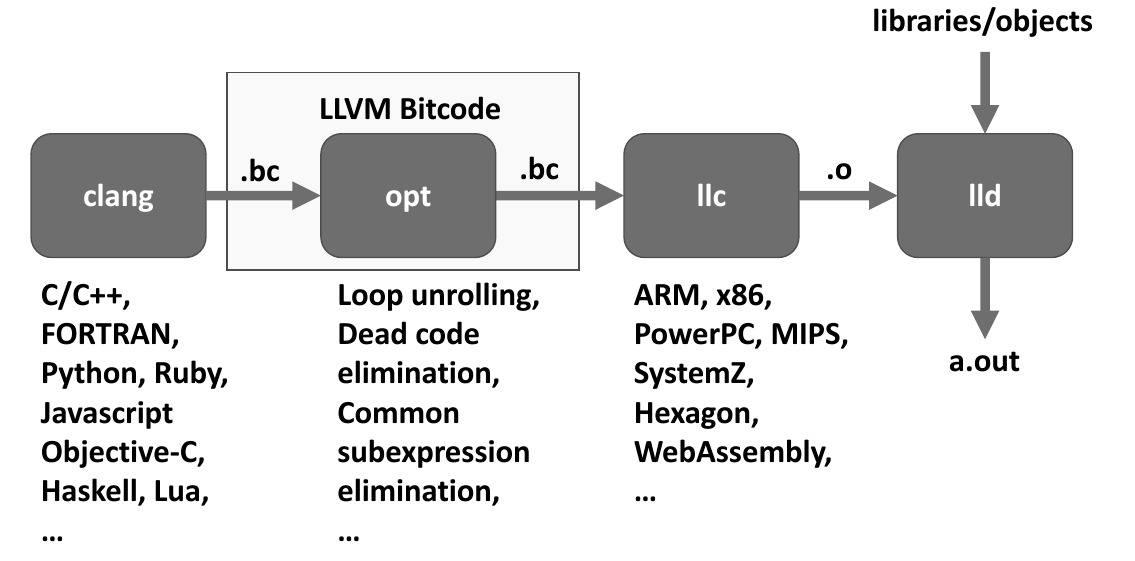
\includegraphics[scale=0.35]{LLVMcompiler.jpg}}
    }
    \caption{Various stages of compilation using Clang}
    \label{fig:LLVMcompiler}
\end{figure}

\section{Common Clang/LLVM Commands}
\label{sec:CommonClangLlvmCommands}

In each of the following commands, an optional output file can be specified using 
\texttt{'-o'} flag.
\begin{itemize} \tightlist
  \item \texttt{'clang hello.c'} - Compiles \textit{hello.c}.
  \item \texttt{'clang++ hello.cpp'} - Compiles \textit{hello.cpp}.
  \item \texttt{'clang -emit-llvm -S hello.c'} - Gives LLVM IR corresponding to \textit{hello.c} in text format file \textit{hello.ll}.
  \item \texttt{'clang -emit-llvm -c hello.c'} - Gives LLVM IR corresponding to \textit{hello.c} in binary bitcode format file \textit{hello.bc}.
  \item \texttt{'llvm-as hello.ll'} - Converts \textit{hello.ll} to \textit{hello.bc}.
  \item \texttt{'llvm-dis hello.bc'} - Converts \textit{hello.bc} to \textit{hello.ll}.
  \item \texttt{'lli hello.bc'} - Directly executes \textit{hello.bc}.
  \item \texttt{'lli hello.ll'} - Directly executes \textit{hello.ll}.
\end{itemize}

\noindent \textbf{NOTE} - Sometimes Clang/LLVM version information is also 
required for running the commands - \texttt{'clang-8', 'clang++-8, 'llvm-as-8', 'llvm-dis-8', 'lli-8'} etc.

\section{Working with Clang/LLVM}
\label{sec:WorkingWithClangLlvm}

This project is done on \textbf{Ubuntu 19.10} operating system using 
\href{https://clang.llvm.org/}{Clang} version 8.0.1 and 
\href{https://llvm.org/}{LLVM} version 8.0.1. The instructions 
mentioned here are verified to work on the same.

\subsection{Installing Clang}
\label{subsec:InstallClang}
First install \href{https://clang.llvm.org/}{Clang} using 
\texttt{'sudo apt-get install'} command. Also, make sure that its 
version is compatible with the version of LLVM to be used.
\smallbreak \noindent \textbf{NOTE} - Install Clang-8 (using 
\texttt{'sudo apt-get install clang-8'}) for working with LLVM-8.0.1.

\subsection{Building LLVM from source}
\label{subsec:BuildingLLVMFromSource}

Before proceeding make sure that \textbf{cmake} is installed on the 
system. For any further help on building LLVM from source, see 
\href{https://llvm.org/docs/CMake.html}{the LLVM documentation page}.

\begin{itemize} \tightlist
    \item First download the LLVM source code from 
    \href{http://releases.llvm.org/download.html}{LLVM download page} 
    or use \href{https://github.com/llvm/llvm-project/releases/download/llvmorg-8.0.1/llvm-8.0.1.src.tar.xz}{this link}
    to download source code for LLVM-8.0.1. 
    \item Extract the LLVM source from the tar-package, at some 
    preferable location. The root folder of the extracted source 
    will now be referred to as \texttt{LLVMsrc}.
    \item Create a new directory, which would be used for building 
    the LLVM source. This directory would be referred to as 
    \texttt{LLVMbuild}.
    \item Run \texttt{'cmake LLVMsrc'} from the \texttt{LLVMbuild} 
    directory. CMake will detect the development environment, perform 
    a series of tests, and generate the files required for building 
    LLVM. 
    \item Run \texttt{'cmake -{}-build .'} from the \texttt{LLVMbuild}
    directory to build the source.

    \textbf{NOTE} - This step might take hours to finish. Also, 
    building has very high memory requirements so it might also fail. 
    In this case repeat the last step and \textit{cmake} would detect 
    the packages it has already built in the previous run, and start 
    from where it was interrupted.
\end{itemize}
        
\subsection{Writing a Pass}
\label{subsec:WritingAPass}
A \textbf{pass} is a program that takes an LLVM IR as input and transforms it
generating a new IR. This new IR can be optimised version of the input or some 
modified version suitable for other tasks. Sometimes a pass only analyses 
the IR without modifying it.
\bigbreak \noindent This section explains how to create a simple pass named \textbf{HelloPass}.
\begin{itemize} \tightlist
    \item Create directory \textit{'LLVMsrc/lib/Transforms/HelloPass'}. This directory will contain files related to the pass.
    \item Create a new file named \textit{helloPass.cpp} inside \textit{HelloPass} directory. This file will contain the code for the pass which is given below.
        \begin{lstlisting}
#include "llvm/ADT/Statistic.h"
#include "llvm/IR/Function.h"
#include "llvm/Pass.h"
#include "llvm/Support/raw_ostream.h"
using namespace llvm;

namespace {
  struct helloPass : public FunctionPass {
    static char ID;
    helloPass() : FunctionPass(ID) {}

    bool runOnFunction(Function &F) override {
      errs() << "Function Name: ";
      errs().write_escaped(F.getName()) << '\n';
      errs() << "===================================================\n";
      for(auto bb = F.begin(); bb != F.end(); bb++){
        errs() << "\tBasicBlock Name = " << bb->getName() << "\n";
        errs() << "\tBasicBlock Size = " << bb->size() << "\n";
        for(auto i = bb->begin(); i != bb->end(); i++){
          errs() << "\t" << "Instruction: " << *i << "\n";
          errs() << "\t" << "OpCode: " << i->getOpcode() << "\n";
          errs() << "\t" << "OpCodeName: " << i->getOpcodeName() << "\n";
          errs() << "\t" << "IsBinaryOp: " << i->isBinaryOp() << "\n";
          errs() << "\t" << "IsCommutative: " << i->isCommutative() << "\n";
          errs() << "\t" << "IsAssociative: " << i->isAssociative() << "\n";
        }
        errs() << "\n\n";
      } 
      return false;
    }
  };
}
char itrinstBB::ID = 0;
static RegisterPass<helloPass> X("hello", 
                                 "Iterates instructions in a function");
        \end{lstlisting}
    The above code contains a \textbf{function pass} - which means the 
    pass is run on every function defined in a file. Using 
    iterators it traverses each basic block of the function, and 
    for each basic block, it traverses each instruction and 
    prints the details of the instruction - like its opcode, 
    whether it is commutative and associative etc.\\
    \textbf{Important} - Notice the first argument \textbf{hello} 
    which is passed in the last line while registering the pass. 
    This argument will be passed as a flag to the 
    \textbf{HelloPass} pass when the function-pass defined inside 
    \textbf{helloPass} structure (the template arguments in the last line)
    is to be executed.
    \item Create a file named \textbf{CMakeLists.txt} in the same 
    HelloPass dirctory. This file will be used by \textbf{make} when 
    building the pass.
        \begin{lstlisting}
add_llvm_library( LLVMhelloPass MODULE
  helloPass.cpp
  PLUGIN_TOOL
  opt
)
        \end{lstlisting}
        \textit{LLVMhelloPass} in the first line specifies the 
        filename (without *.so extension) inside \textit{'LLVMbuild/lib/'}
        directory, which will contain the pass when built. 
        \textit{helloPass.cpp} in the second line specifies the file 
        which contains the source code for the pass.
    \item Add the following line to the file 
    \textit{'LLVMsrc/lib/Transforms/CMakeLists.txt'}
        \begin{lstlisting}
add_subdirectory(HelloPass)
        \end{lstlisting}
    This is the name of folder which contains the files related to the pass 
    and will also be used by \textbf{make} while building.

\end{itemize}

\textbf{NOTE} - More detailed tutorial on writing a pass can be found 
\href{http://llvm.org/docs/WritingAnLLVMPass.html#quick-start-writing-hello-world}{here}.

\subsection{Running the pass}
\label{subsec:RunningThePass}
\begin{itemize} \tightlist
    \item Rebuild the LLVM source so that it includes the new
    pass that was added. For this change current directory to \textit
    {LLVMbuild} and run \texttt{'make'}.
    \item Now run the pass on a binary bitcode file \textit{source.bc}, 
    containing an LLVM IR as \\
    \texttt{'./bin/opt -load ./lib/LLVMhelloPass.so -hello source.bc -o sourceN.bc'}.\\
    The pass can also be run on a \texttt{'*.ll'} file in a similar way.
    
  \end{itemize}
  
\noindent \textbf{NOTE} - \texttt{'LLVMhelloPass'} is the same name that was
specified in the \textit{CMakeLists.txt} file of the pass folder. Also, 
\texttt{'-hello'} flag is the name by which the pass was registered.

\cleardoublepage
\typeout{}
\chapter{LLVM Implementation of the Algorithm}
\label{chap:chapter7}

This chapter provides details of implementation of the Herbrand equivalence 
algorithm for Clang/LLVM compiler framework. The actual implementation along 
with other details like how to run and how to interpret the output etc. can be 
found on \href{https://github.com/himanshu520/HerbrandEquivalence/tree/master/LLVM}{GitHub} 
and for extensive documentation refer to \href{https://himanshu520.github.io/HerbrandEquivalenceLLVMDocs/}{LLVMDocs}.

\section{LLVM Intermediate Representation (IR)}
\label{sec:LLVMIntermediateRepresentation}

Performing analysis and optimizations on a high level language code is very 
difficult. So compilers first convert the high level code to some intermediate 
representation. An IR is designed to be closer to assembly language yet 
independent of the target machine. It is designed such that the analysis and 
optimizations can be performed more conviniently compared to doing the same on 
the high level language. IRs are usually abstract internal representations 
rather than actual language.

LLVM IR is the intermediate form used by LLVM. Rather than just being an abstract
internal representation, LLVM is a complete language on its own. It even provides 
human-readable assembly format for the IR. To get readable IR corresponding to 
file \textit{hello.c}, run \texttt{'clang-8 -emit-llvm -S hello.c -o hello.ll'}. 
The IR file can also be directly executed as \texttt{'lli hello.ll'}.

Apart from already existing optimizations in LLVM, one can write their own 
optimizations/analysis programs called \textbf{LLVM passes}. This chapter 
discusses the details of the pass written to perform Herbrand equivalence 
analysis. A brief tutorial on writing a basic pass is already covered in 
\autoref{sec:WorkingWithClangLlvm}.

\subsection{Basics of LLVM IR}
\label{subsec:BasicsOfLlvmIr}
\begin{itemize} \tightlist
    \item The temporaries and labels in LLVM IR has no name; however in \textit{*.ll} files they are named as \texttt{\%0, \%1, \%2, ...}. But for reference names can be assigned to them.
    \item All the local variables in a function are allocated space on the stack using \texttt{alloca} instruction in the beginning of the function itself. Pointers to these locations are assigned to temporaries in order to allow access to them.
    \item Each time a value is assigned to be a local variable, it is updated immediately on the stack using its corresponding temporary with \texttt{store} instruction. Similarly each time a variable's value is to be accessed, it is loaded into a new temporary using \texttt{load} instruction.
    \item The result of every computation is stored in a new temporary and these temporaries can be assigned values only once. The values assigned to actual program variables (stored on stack) can be changed indirectly through their pointers; but the temporaries actually holding the pointers are also not reassignable.
    \item Example - Consider the instruction \texttt{x = y + z} and suppose that \texttt{\%0, \%1, \%2} holds the stack locations allocated to \texttt{x, y, z} respectively. This single instruction would correspond to four instructions in the IR. First load the values of \texttt{y} and \texttt{z} in new temporaries \texttt{\%3} and \texttt{\%4}; \texttt{\%5} is assigned \texttt{\%3 + \%4} and finally the value in \texttt{\%5} is stored in location pointed by \texttt{\%0}.
    \item Constants and temporaries are of type \texttt{Value} in LLVM and they can be accessed through pointers (of type \texttt{Value*}). Instructions are of type \texttt{Instruction} which itself is derived from class \texttt{Value}. Functions have type \texttt{Function}.
\end{itemize}

\paragraph{NOTES} 
\begin{itemize}
    \item In the implementation, for stack variables - the temporaries storing their addresses have been taken to represent the actual variables themselves. This way from the implementation point of view, such temporaries can change their values.
    \item The temporaries in the output are named as \texttt{T1, T2, ...}
\end{itemize}

\section{\texttt{Herbrand Equivalence Pass}}
\label{sec:HerbrandEquivalencePass}

\subsection{Data Structures}
\label{subsec:DataStructuresLLVM}
\begin{itemize} \tightlist
    \item \texttt{ExpressionTy} - \texttt{std::tuple<char, Value*, Value*>} to represent an expression.
    \item \texttt{CfgNodeTy} - Represents a control flow graph node and has following data members -
        \begin{itemize}
            \item \texttt{NodeTy} - \texttt{Enum} to denote the kind of node - \texttt{START}, \texttt{END}, \texttt{TRANSFER}, \texttt{CONFLUENCE}.
            \item \texttt{instPtr} - \texttt{Instruction*} pointing to the instruction that defines the transfer function if the node corresponds to a transfer point.
            \item \texttt{predecessors} - \texttt{std::vector<int>} containing indexes of predecessor control flow graph nodes (see \texttt{CFG}).
        \end{itemize}
\end{itemize}

\subsection{Global Variables}
\label{subsec:GlobalVariablesLLVM}
\begin{itemize} \tightlist
    \item \texttt{Constants} - \texttt{std::set<Value*>} storing the constants used in the program.
    \item \texttt{Variables} - \texttt{std::set<Value*>} storing the variables used in the program.
    \item \texttt{Ops} - \texttt{std::set<char>} storing the operands appearing in the programs on which the pass is run.
    \item \texttt{IndexExp} - \texttt{std::map<ExpressionTy, int>} to map program expressions of length atmost two to integers for indexing purpose.
    \item \texttt{SetCnt} - Next set identifier to be used.
    \item \texttt{Partitions} - \texttt{std::vector<std::vector<int>>} to keep track of partition at each program point. \texttt{Partitions[v][n]} stores the set identifier each expression \texttt{e} such that \texttt{IndexExp[e]} is \texttt{n}, at program point represented by \texttt{CFG[v]}. Also, \texttt{Partitions[v]} is the \textbf{partition vector} representing the partition at program point \texttt{CFG[v]} (see \texttt{CFG}).
    \item \texttt{Parent} - \texttt{std::map<std::tuple<char, int, int>, int>} to store parent set identfiers.
    \item \texttt{CFG} - \texttt{std::vector<CfgNodeTy>} to store program control flow graph.
    \item \texttt{CfgIndex} - \texttt{std::map<Instruction*, int>} to store the index of control flow graph node corresponding to instructions in the program, for which they define the transfer function (see \texttt{CFG}).
\end{itemize}
\textbf{NOTE} - For more details on \texttt{SetCnt}, \texttt{Partitions} and \texttt{Parent} refer to \autoref{sec:NotationPseudocode}.

\subsection{Functions}
\label{subsec:FunctionsLLVM}
\begin{itemize} \tightlist
    \item \texttt{assignNames(F)} - Assign names to basic blocks and  temporaries in function \texttt{F} for easy reference.
    \item \texttt{assignIndex(F)} - First iterates over instructions in function \texttt{F} to update \texttt{Constants} and \texttt{Variables}. Then updates \texttt{IndexExp} assigning integer indexes to expressions (of length atmost two) arbitrarily at the beginning of the analysis, for indexing purpose.
    \item \texttt{createCFG(F)} - Creates control flow graph corresponding to function \texttt{F} by updating \texttt{CFG}.
    \item \texttt{printValue(v)} - Function to print a constant or a variable (of type \texttt{Value*}) in a readable format.
    \item \texttt{printExpression(e)} - Function to print expression \texttt{e} (of type \texttt{ExpressionTy}) in a readable format.
    \item \texttt{printCode(F)} - Prints function \texttt{F} in a readable format.
    \item \texttt{printCFG()} - Prints control flow graph in readable format (see \texttt{CFG}).
    \item \texttt{printPartition(p)} - Prints partition vector \texttt{p} (of type \texttt{std::vector<int>}) in a readable format.
    \item \texttt{samePartition(p1, p2)} - Checks if the two partition vectors (\texttt{std::vector<int>}) \texttt{p1} and \texttt{p2} are same. They are same when values (ie. set identifiers) at two different indexes are equal in the first iff they are so in the second.
    \item \texttt{findSet(p, e)} - Finds set identifier representing expression \texttt{e} (which is of type \texttt{ExpressionTy}) in partition vector \texttt{p}.
    \item \texttt{findInitialPartition(p)} - Intialises partition vector \texttt{p} with $\bot$.
    \item \texttt{getClass(p, n, c)} - Updates \texttt{c} (\texttt{std::set<int>}) to contain indexes of expressions which are equivalent to expression with index \texttt{n}, in the partition vector \texttt{p}.
    \item \texttt{transferFunction(n)} - Applies corresponding transfer function to the partition at program point \texttt{CFG[n]}.
    \item \texttt{confluenceFunction(n)} - Applies the confluence operation to the partition at program point \texttt{CFG[n]}.
    \item \texttt{HerbrandAnanlysis(F)} - Performs Herbrand analysis over function \texttt{F}.
\end{itemize}

\bigskip \noindent \textbf{NOTE} - For more details on the function implementation, refer to \autoref{chap:chapter4} and for extensive documentation refer to \href{https://himanshu520.github.io/HerbrandEquivalenceLLVMDocs/}{LLVMDocs}.

\section{Benchmarking}
\label{sec:Benchmarking}

The idea was to use the analysis information to perform program optimizations - like constant propagation, constant folding, common subexpression elimination etc. These optimizations were to be benchmarked using \href{https://www.spec.org/}{SPEC benchmarking suites}. The SPEC establishes, maintains and endorses standardized benchmarks and tools to evaluate performance and energy efficiency for the newest generation of computing systems. In particular \textbf{SPEC CPU benchmarks} are used for measuring and comparing compute intensive performance, stressing a system's processor, memory subsystem and \textit{compilers}. Here, the CPU benchmarks were to be used for comparing the performance of our optimizations with respect to ones already existing like common subexpression elimination, global value numbering both in terms of processing time (time taken to optimize a program) and execution time (of the optimized program).

The SPEC test cases are actual real world programs with slight modifications focussing on the kind of benchmarks to be done; some of these includes GCC, Perl interpreter, video compression program etc. These are large programs and for an optimization pass to be successfully benchmarked, it must be able to correctly handle all the constructs in LLVM IR. One must know how the high level language constructs like different basic types, pointers, classes, unions, enumerations etc. are translated in the IR; how to operate with them in the IR; and what are the feasible modifications that can be peformed without breaking the consistency and correctness of the programs. In short, one must have very deep and extensive knowledge of LLVM. This is very difficult given the size of the LLVM project itself and limited tutorials available and even the ones available are very basic. Though the documentation is extensive, it is useful only as a reference and is of not much use to a know-nothing.

The current implementation has many limitations. It considers only integer variables and doesn't expect other basic types like floats, boolean, characters etc. Also it can't handle derived and complex types like structures, classes, unions, enumerations, pointers etc. It considers only five arithematic operators - \texttt{+, -, *, /, \%}.

Though some of these can be easily handled, there are still others and the ones not mentioned like handling global variables, recursion, dynamic memory allocation etc. Given these complications it was decided to leave the implementation as such and skip the benchmarkings.

\cleardoublepage
\typeout{}
\chapter{Performing Optimizations}
\label{chap:chapter8}

This chapter explains how to use the Herbrand Equivalence analysis
information to perform actual program optimizations.

\section{Available Variables}
\label{AvailableVariables}
A variable is said to be \textbf{available} at a basic block if 
it is defined at some point along all the execution paths from the 
start of the program that reaches the beginnning of that basic block.
It is forward data analysis problem and can be determined via fixed 
point computation.

The universe $\mathcal U$ would be the set of all program variables.
Also, let $\mathcal B$ be the set of all basic blocks in the program.
Denote by $DEF[B]$ the set of variables defined in the basic block
$B \in \mathcal B$, and $IN[B]$ be corresponding set of available 
variables. Initialise $OUT[B] = \mathcal U, \forall B \in \mathcal B$ 
and perform updates as follows till a fixed point is reached.
$$IN[B] = \cap_{B' \in Predecessors(B)} OUT[B']$$
$$OUT[B] = IN[B] \cup DEF[B]$$

Note that the definition of \textbf{available variables} is different
from that of \textbf{reaching definitions} and \textbf{available 
expressions}. If a variable is available at the beginning of a given
basic block, then that variable can be used in the basic block without
defining it because by \textit{definition of avilable variables} it 
would already be defined along every path from the start of the 
program to that basic block.

The definition of available variables can be extended to that of any
instruction. Variables available at an instruction $I$ is the union 
of variables available at the beginning of its basic block and any 
variables defined by the instructions preceding it in that block.

\section{Performing Optimizations}
\label{PerformingOptimizations}
The results of Herbrand Equivalence and available variables analysis 
can be used to perform optimizations involving redundant expression 
elimination and some dead code elimination.

Suppose, there is an instruction $I : z \gets e$, where $e$ is an 
expression (as already mentioned expression means either a constant, 
or a variable or a length two expression). First find the Herbrand 
equivalence class of $z$ at that program point. If the class represents
a constant valued expression ($partitions[I][z].isConst == true$), then
this instruction can be deleted and all uses of $z$ replaced by 
$partitions[I][z].constVal$, till $z$ is redefined. Else if it is not 
a constant valued expression, 
$\mathcal S = (getClass(partitions[I], z) \cap IN[I])$
will be the set of variables, such that $z$ can be replaced by 
$s \in \mathcal S$ (before $z$ and $s$ are redefined), without changing
the meaning of the program. \\ 
Pseudocode \ref{Optimize} is the precise formulation of the mentioned facts.

\begin{algorithm}
\caption{Performing Optimizations}\label{Optimize}
\begin{algorithmic}[1]
\Procedure{Optimize}{}
    \For{$B \in \mathcal B$}
        \State $Insts \gets$ \textbf{Instructions}$(B)$
        \State $AvailVars \gets IN[B]$
        \State
        \For{$I \in Insts$}
            \State $Insts.remove(I)$
            \State $z \gets$ \textbf{LValue}$(I)$
\algstore{Optimize}
\end{algorithmic}
\end{algorithm}
                    

\begin{algorithm}
\begin{algorithmic}[1]
\algrestore{Optimize}
            \If{\textbf{Defined}$(z)$}
                \State \textbf{IDstruct*} $ptr \gets partitions[I][z]$
                \State
                \If{$ptr.isConst$}
                    \State \textbf{Bool} $reachedEnd \gets true$
                    \For{$I' \in Insts$}
                        \If{\textbf{LValue}$(I') == z$}
                            \State $reachedEnd \gets false$
                            \State \textbf{break}
                        \EndIf
                        \State \textbf{Replace}$(I',\ z,\ ptr.constVal)$
                    \EndFor
                    \If{$reachedEnd$}
                        \State $B.insert(z \gets ptr.constVal)$
                    \EndIf
                    \State
                    \State \textbf{DeleteInstruction}$(I)$
                \Else
                    \State \textbf{set}$<$\textbf{Expressions}$> curPart \gets$ \textbf{GetClass}$(partitions[I],\ z)$
                    \State $curPart \gets (curPart \cap AvailVars)$
                    \State
                    \If{not $curPart.empty()$}
                        \State \textbf{Bool} $reachedEnd \gets true$
                        \State $replacement \gets curPart.first()$
                        \State
                        \For{$I' \in Insts$}
                            \If{\textbf{LValue}$(I') == z$}
                                \State $reachedEnd \gets false$           
                                \State \textbf{break}
                            \EndIf
                            \State $curPart = curPart \setminus \{$\textbf{LValue}$(I')\}$
                            \If{not $curPart.empty()$}
                                \State $replacement \gets curPart.first()$
                                \State \textbf{Replace}$(I',\ z,\ replacement)$
                            \Else
                                \State $B.insert(I', z \gets replacement)$
                                \State $AvailVars \gets AvailVars \cup \{z\}$
                                \State $reachedEnd \gets false$
                                \State \textbf{break}
                            \EndIf
                        \EndFor
                        \State
                        \If{$reachedEnd$}
                            \State $B.insert(z \gets replacement)$
                        \EndIf
                        \State \textbf{DeleteInstruction}$(I)$
                        \State
                    \Else
                        \State $AvailVars \gets AvarilVars \cup \{z\}$
                    \EndIf
                \EndIf
            \EndIf
        \EndFor
    \EndFor
\EndProcedure
\end{algorithmic}
\end{algorithm}
    
Also note the following functions whose details has not been provided.\\
\textbf{Instructions}$(B)$ :- Returns a list of instructions in the basic block $B$.\\
\textbf{Replace}$(I', z, replacement)$ :- Replaces variable $z$ in the instruction $I'$ with $replacement$ which can be a constant or another variable.\\
\textbf{B.insert}$(I)$ :- Inserts instruction $I$, at the end of basic block $B$.\\
\textbf{B.insert}$(I, I')$ :- Insert instruction $I'$ before instruction $I$ in basic block $B$.\\
\textbf{DeleteInstruction}$(I)$ :- Deletes instruction $I$ from the program.\\
\textbf{set.empty}$()$ :- Returns $true$ if $set$ is empty, else $false$.\\
\textbf{set.first}$()$ :- Returns first element from $set$.\\

\section{LLVM Implementation}
\label{LLVMImplementation}
The LLVM specific implementation of the pseudocodes mentioned can be found in 
\href{https://github.com/himanshu520/HerbrandEquivalence}{this github repository}.
\cleardoublepage
\typeout{}
\chapter{Proof Attempt}
\label{chap:chapter9}

\autoref{sec:AugmentedProgramApproach} contains details of the attempt made to prove the correctness of the algorithm - reason for the mentioned approach, claims made and reasons for its failure. \autoref{sec:WhyTheAlgorithmWorks} informally shows why the algorithm should work for the special case when the input program has no loops.

\section{Augmented Program Approach}
\label{sec:AugmentedProgramApproach}
Let $\mathcal{X}$ and $\mathcal{I}$ be the set of variables and instructions in the program respectively. Also, let $\mathcal{T}$ and $V$ be the set of terms and program points; and $\mathcal{D}(V, \mathcal{F})$ be the corresponding data flow framework. Let $\mathcal{W} \subseteq \mathcal{T}$ be the corresponding set of terms of length atmost two (in terms of number of operands).

The basic motive behind this approach was to prevent the disappearance of some equivalence classes in between the program due to reassignment to variables (see \autoref{sec:tc4} for an example). The classes disappear because there exists no expression in our working set $\mathcal{W}$ that belongs to that class however that class still contains expressions outside $\mathcal{W}$.

\subsection{Augmented Program}
\label{subsec:AugmentedProgram}

Every instruction in the original program is extended to a \textbf{bundle} of instructions - for each instruction $i \in \mathcal{I}$, add immediately after it dummy instructions of the form $x_i \gets x, \forall x \in \mathcal{X}$. This new program with dummy instructions is called the \textbf{augmented program} and the new variables introduced are called \textbf{shadow variables}.
\\
Let $\overline{\mathcal{X}}$, $\overline{\mathcal{I}}$, $\overline{\mathcal{T}}$ and $\overline{V}$ be the corresponding sets of variables, instructions, terms and program points respectively; and $\overline{\mathcal{D}}(\overline{V}, \overline{\mathcal{F}})$ be the corresponding data flow framework. Also $\overline{\mathcal{W}} \subseteq \overline{\mathcal{T}}$ be the corresponding set of terms restricted to length atmost two.

\subsection{Idea}
\label{subsec:Idea}
Let $\mathcal{L}$ and $\overline{\mathcal{L}}$ be the infinite lattices associated with the original and augmented programs respectively. These are same as $\overline{\mathcal{G}(\mathcal{T})}$ described in \autoref{sec:CongruenceRelation}, for the original and augmented programs.
\\
Given a partition $\mathcal{P}$, define 
$$\Phi_W(\mathcal{P}) = \{A_i \cap W \mid A_i \in \mathcal{P} \ \mathrm{and} \ (A_i \cap W) \neq \phi\}$$
Let $\Phi_W$ be generalised so that when applied to set of partitions $\mathcal{S}$,
$$\Phi_W(\mathcal{S}) = \{\Phi_W(\mathcal{P}) \mid \mathcal{P} \in \mathcal{S}\}$$
It is clear that $\mathcal{L} = \Phi_{\mathcal{T}}(\overline{\mathcal{L}})$. Let $\mathcal{L}_{\mathcal{W}} = \Phi_{\mathcal{W}}(\mathcal{L})$ and $\overline{\mathcal{L}}_{\overline{\mathcal{W}}} = \Phi_{\overline{\mathcal{W}}}(\overline{\mathcal{L}})$ be the finite lattices associated with the original and augmented lattices respectively.
\\
Let $f_{\mathcal{D}}$ and $\overline{f}_{\overline{\mathcal{D}}}$ be be the composite transfer function associated $\mathcal{L}$ and $\overline{\mathcal{L}}$ respectively, as defined in \autoref{chap:chapter3}. The Hebrand congruence functions are given by 
$$\mathcal{H}_{\mathcal{D}} = \bigwedge \{\top, f_{\mathcal{D}}(\top), f_{\mathcal{D}}^2(\top), ...\}\ \mathrm{and}\ \overline{\mathcal{H}}_{\overline{\mathcal{D}}} = \bigwedge \{\overline{\top}, \overline{f}_{\overline{\mathcal{D}}}(\overline{\top}), \overline{f}_{\overline{\mathcal{D}}}^2(\overline{\top}), ...\}$$
for the original and augmented lattice. Here, $\top$ and $\overline{\top}$ stands for top element in the product lattices corresponding to $\mathcal{L}$ and $\overline{\mathcal{L}}$ respectively.

\subsubsection{Observations}
\label{subsubsec:Observations}
\begin{itemize}
    \item $\Phi_{\mathcal{W}}(\mathcal{H}_{\mathcal{D}}) = \Phi_{\mathcal{W}}(\overline{\mathcal{H}}_{\overline{\mathcal{D}}})$
    \item $\Phi_{\mathcal{W}}(\Phi_{\overline{\mathcal{W}}}(\overline{\mathcal{H}}_{\overline{\mathcal{D}}})) = \Phi_{\mathcal{W}}(\mathcal{H}_{\mathcal{D}})$
\end{itemize}

\subsubsection{Claim}
\label{subsubsec:Claim}
$$\Phi_{\overline{W}}(\overline{\mathcal{H}}_{\overline{\mathcal{D}}}) =\text{ Maximum fix point of transfer function } \overline{f}_{\overline{\mathcal{W}}} \text{ on } \overline{\mathcal{L}}_{\overline{\mathcal{W}}}$$
The right hand side can computed efficiently using the algorithms in \autoref{chap:chapter4}, on the augmented program.

\subsection{Hypothesis}
\label{subsec:Hypothesis}
Following hypothesis was proposed which was supposed to be used later to prove the claim - suppose at program point $v \in V$ in the original program, variable $x \cong t$ (where $\mid t \mid\ \geq 2$) in our original infinite lattice $\mathcal{L}$, then at the output of the bundle corresponding to program point $v$ in the augmented program, there exists $t'$ in augmented finite lattice $\overline{\mathcal{L}}_{\overline{\mathcal{W}}}$ with $\mid t' \mid\ = 2$ which is equivalent to $x$ and consists only of constants and shadow variables.
\\
However, a counter example to the hypothesis was discovered while attempting the proof for the hypothesis. Consider test case in \autoref{sec:tc13} - at the confluence point (program point 6), in the original infinite lattice $x$ and $((y + z) + n)$ are equivalent; but in the augmented finite lattice no two length expression consisting of only shadow variables and constants that is equivalent to $x$.

\section{Why the Algorithm Works}
\label{sec:WhyTheAlgorithmWorks}
Instead of a general case, consider the ones in which the program has no loops. In such cases the control flow graph (CFG) is a directed acyclic graph (DAG). And if the algorithm processes CFG nodes in the topological order, it converges in the first iteration itself.

The \texttt{Parent} map captures the syntactic information present in the expressions in the form of an ordered tree. Each node in the tree is assigned a unique set identifier and represents some syntactically equivalent expressions. Suppose a node has set identifier $x$ and \texttt{Partitions[v][e]} is $x$ - it means that at program point $v$, expression $e$ has same syntactic value (across all program paths from the start) as represented by the node. A node captures this syntactic information in the form of its two ordered childrens and an operator - which is precisely the information stored the \texttt{Parent} map. Leaf nodes represents atomic values - a constant, non-deterministic or variable (variable in terms of different values along different execution paths) value. These properties implies that two expressions that are assigned the same set identifier at a program point are Herbrand equivalent at that point, which shows the correctness of the algorithm.

Now induction can be used to show that the algorithm actually maintains the properties mentioned in the last paragraph when it processes the nodes in the topological order.
\\
At the \texttt{START} point all the expressions in $\mathcal{W}$ are inequivalent to each other. And the algorithm also assigns different set identifiers to elements of $\mathcal{W}$. Also, for all $x_1 + x_2 \in (\mathcal{W} \setminus (\mathcal{C} \cup \mathcal{X}))$, \texttt{Parent[\{+, Partitions[START][$x_1$], Partitions[START][$x_2$]\}]} is assigned \texttt{Partitions[START][$x_1 + x_2$]}. So the properties hold at \texttt{START} point.

Now the properties will be shown to hold for program point $v$, assuming that they hold at all points which occur before $v$ in the topological order - in particular they hold for all $u \in \texttt{Predecessors[v]}$.
\begin{itemize}
    \item \textbf{$v$ is a transfer point}\\
    Suppose $v$ represents the assignment $x = e$ and $u$ is its predecessor. With respect to $u$, the only expressions changing values are the ones which contain $x$. So \texttt{Partitions[u]} is copied to \texttt{Partitions[v]} and $x$ is assigned the set identifier of $e$ because they now have equal values.\\
    Now consider all expressions of the form $a + b$ which contains $x$. If \texttt{Parent[\{+, Partitions[v][a], Partitions[v][b]\}]} is defined it means that there already exists a node that represents expressions syntactically equivalent to the value of $a + b$ at the current point. So \texttt{Partitions[v][a + b]} should be assigned the same set identifier. However, if no such node exists a new one needs to be created and is to be assigned to \texttt{Parent[\{+, Partitions[v][a], Partitions[v][b]\}]} as well as to \texttt{Partitions[v][a + b]} to maintain the properties. This is consistent with what the algorithm actually does.

    \item \textbf{$v$ is a confluence point}\\
    If $e \in \mathcal{W}$ has same set identifiers for all $u \in \texttt{Predecessors[v]}$, it means that it has same syntactic value at all its predecssors and hence even at the confluence point - so it must be assigned the same set identifier (as that of the predecessors) even at $v$ to maintain the properties.\\
    However, if $e \in \mathcal{W}$ has different identifiers at the predecessors then not all the values at the predecessor points are syntactically equivalent - for this case we require a new leaf node (because of variable values at predecessors). So we must find expressions which are equivalent to $e$ at all the predecessors - and assign a new set identifier (new leaf node) for them to maintain the properties.\\
    These both cases are consistent with the algorithm.
\end{itemize}

\cleardoublepage
\typeout{}
\chapter{Conclusion}
\label{chap:chapter10}
Detection of equivalent expressions in a program can be used in multiply ways - compilers can use it for program optimisations involving redundant expression elimination, dead code elimination etc.; in program verification and plagiarism detection tools etc. So Herbrand equivalence being a form of equivalent expression analysis has a huge importance both from theoretical as well as practical point of view.

\section{Summary of Work Done}
\label{sec:SummaryOfWorkDone}
\begin{itemize}
    \item Pointed out few errors in the original alogrithm proposed by Babu et al. 
    \cite{Babu} and refined it making it more efficient than the original
    version (see \autoref{sec:UpdatesOverOriginalAlgorithm}). The new updated
    algorithm is given in \autoref{chap:chapter4}.
    \item Completed LLVM implementation (see \autoref{chap:chapter7}) and the code for the same can be found on \href{https://github.com/himanshu520/HerbrandEquivalence/tree/master/LLVM}{GitHub}.
    Benchmarking was skipped as it is not feasible (see \autoref{sec:Benchmarking}).
    \item In addition to LLVM implementation an additional implementation for
    a toy language is done (see \autoref{chap:chapter8}) and its code can also 
    be found on \href{https://github.com/himanshu520/HerbrandEquivalence/tree/master/ToyLanguage}{GitHub}.
    \item An attempt for proving the algorithm (see \autoref{chap:chapter9}) 
    was made but it failed because counterexample to a hypothesis was found that was supposed to be used later in the final proof
    (see \autoref{subsec:Hypothesis}). However an informal proof of why the 
    algorithm should work is given in \autoref{sec:WhyTheAlgorithmWorks}, 
    for special case when the input program has no loops.
\end{itemize}

\section{Future Scope}
Though the algorithm gives correct results for the test cases on which it was tried, work for complete formal proof of its correctness is still ongoing. The algorithm is already efficient being polynomial in time with respect to the program size; so once the correctness is proven it can easily be employed for different applications mentioned earlier.
\cleardoublepage

\let\cleardoublepage\clearpage
\addcontentsline{toc}{chapter}{External References}
\raggedbottom
\doublespacing
\chapter*{External References}
\vskip 2ex 

\begin{itemize}
    \item \textbf{GitHub repository for the project}\\
    \href{https://github.com/himanshu520/HerbrandEquivalence}{\texttt{github.com/himanshu520/HerbrandEquivalence}}
    \item \textbf{Documentation for LLVM implementation}\\
    \href{https://himanshu520.github.io/HerbrandEquivalenceLLVMDocs/}{\texttt{himanshu520.github.io/HerbrandEquivalenceLLVMDocs/}}
    \item \textbf{Documentation for toy language implementation}\\
    \href{https://himanshu520.github.io/HerbrandEquivalenceToyDocs/}{\texttt{himanshu520.github.io/HerbrandEquivalenceToyDocs/}}
    \item \textbf{LLVM download page}\\
    \href{http://releases.llvm.org/download.html}{\texttt{releases.llvm.org/download.html}}
    \item \textbf{Source code for LLVM-8.0.1}\\
    \href{https://github.com/llvm/llvm-project/releases/download/llvmorg-8.0.1/llvm-8.0.1.src.tar.xz}{\texttt{github.com/llvm/llvm-project/releases/download/llvmorg-8.0.1/}}\\\href{https://github.com/llvm/llvm-project/releases/download/llvmorg-8.0.1/llvm-8.0.1.src.tar.xz}{\texttt{llvm-8.0.1.src.tar.xz}}
    \item \textbf{LLVM language reference manual}\\
    \href{https://llvm.org/docs/LangRef.html}{\texttt{llvm.org/docs/LangRef.html}}
    \item \textbf{Tutorial for writing an LLVM pass}\\
    \href{https://llvm.org/docs/WritingAnLLVMPass.html}{\texttt{llvm.org/docs/WritingAnLLVMPass.html}}
\end{itemize}

\bibliographystyle{IEEEtran}
\bibliography{citations}
\end{document}
